\documentclass{sigchi}

% Use this section to set the ACM copyright statement (e.g. for
% preprints).  Consult the conference website for the camera-ready
% copyright statement.

% Copyright
\CopyrightYear{2016}
%\setcopyright{acmcopyright}
\setcopyright{acmlicensed}
%\setcopyright{rightsretained}
%\setcopyright{usgov}
%\setcopyright{usgovmixed}
%\setcopyright{cagov}
%\setcopyright{cagovmixed}
% DOI
\doi{http://dx.doi.org/10.475/123_4}
% ISBN
\isbn{123-4567-24-567/08/06}
%Conference
\conferenceinfo{CHI'18,}{May 07--12, 2016, San Jose, CA, USA}
%Price
\acmPrice{\$15.00}

% Use this command to override the default ACM copyright statement
% (e.g. for preprints).  Consult the conference website for the
% camera-ready copyright statement.

%% HOW TO OVERRIDE THE DEFAULT COPYRIGHT STRIP --
%% Please note you need to make sure the copy for your specific
%% license is used here!
% \toappear{
% Permission to make digital or hard copies of all or part of this work
% for personal or classroom use is granted without fee provided that
% copies are not made or distributed for profit or commercial advantage
% and that copies bear this notice and the full citation on the first
% page. Copyrights for components of this work owned by others than ACM
% must be honored. Abstracting with credit is permitted. To copy
% otherwise, or republish, to post on servers or to redistribute to
% lists, requires prior specific permission and/or a fee. Request
% permissions from \href{mailto:Permissions@acm.org}{Permissions@acm.org}. \\
% \emph{CHI '16},  May 07--12, 2016, San Jose, CA, USA \\
% ACM xxx-x-xxxx-xxxx-x/xx/xx\ldots \$15.00 \\
% DOI: \url{http://dx.doi.org/xx.xxxx/xxxxxxx.xxxxxxx}
% }

% Arabic page numbers for submission.  Remove this line to eliminate
% page numbers for the camera ready copy
% \pagenumbering{arabic}

% Load basic packages
\usepackage{balance}       % to better equalize the last page
\usepackage{graphics}      % for EPS, load graphicx instead 
\usepackage[T1]{fontenc}   % for umlauts and other diaeresis
\usepackage{txfonts}
\usepackage{mathptmx}
\usepackage[pdflang={en-US},pdftex]{hyperref}
\usepackage{color}
\usepackage{booktabs}
\usepackage{textcomp}
\usepackage{float}

% Some optional stuff you might like/need.
\usepackage{microtype}        % Improved Tracking and Kerning
% \usepackage[all]{hypcap}    % Fixes bug in hyperref caption linking
\usepackage{ccicons}          % Cite your images correctly!
% \usepackage[utf8]{inputenc} % for a UTF8 editor only

% If you want to use todo notes, marginpars etc. during creation of
% your draft document, you have to enable the "chi_draft" option for
% the document class. To do this, change the very first line to:
% "\documentclass[chi_draft]{sigchi}". You can then place todo notes
% by using the "\todo{...}"  command. Make sure to disable the draft
% option again before submitting your final document.
\usepackage{todonotes}

% Paper metadata (use plain text, for PDF inclusion and later
% re-using, if desired).  Use \emtpyauthor when submitting for review
% so you remain anonymous.
\def\plaintitle{Learning Technique for Optimized Keyboards }
\def\plainauthor{First Author, Second Author, Third Author,
  Fourth Author, Fifth Author, Sixth Author}
\def\emptyauthor{}
\def\plainkeywords{Authors' choice; of terms; separated; by
  semicolons; include commas, within terms only; required.}
\def\plaingeneralterms{Documentation, Standardization}

% llt: Define a global style for URLs, rather that the default one
\makeatletter
\def\url@leostyle{%
  \@ifundefined{selectfont}{
    \def\UrlFont{\sf}
  }{
    \def\UrlFont{\small\bf\ttfamily}
  }}
\makeatother
\urlstyle{leo}

% To make various LaTeX processors do the right thing with page size.
\def\pprw{8.5in}
\def\pprh{11in}
\special{papersize=\pprw,\pprh}
\setlength{\paperwidth}{\pprw}
\setlength{\paperheight}{\pprh}
\setlength{\pdfpagewidth}{\pprw}
\setlength{\pdfpageheight}{\pprh}

% Make sure hyperref comes last of your loaded packages, to give it a
% fighting chance of not being over-written, since its job is to
% redefine many LaTeX commands.
\definecolor{linkColor}{RGB}{6,125,233}
\hypersetup{%
  pdftitle={\plaintitle},
% Use \plainauthor for final version.
%  pdfauthor={\plainauthor},
  pdfauthor={\emptyauthor},
  pdfkeywords={\plainkeywords},
  pdfdisplaydoctitle=true, % For Accessibility
  bookmarksnumbered,
  pdfstartview={FitH},
  colorlinks,
  citecolor=black,
  filecolor=black,
  linkcolor=black,
  urlcolor=linkColor,
  breaklinks=true,
  hypertexnames=false
}

\newcommand{\textred}[1]{\textcolor{red}{#1}}
\ifx\noeditingmarks\undefined
\newcommand{\pgwrapper}[2]{\textred{#1 #2}}
\else
\newcommand{\pgwrapper}[2]{}
\fi
\newcommand{\jl}[1]{\pgwrapper{[JL]}{#1}}
\newcommand{\gdc}[1]{\pgwrapper{[GDC]}{#1}}

% create a shortcut to typeset table headings
% \newcommand\tabhead[1]{\small\textbf{#1}}

% End of preamble. Here it comes the document.
\begin{document}

\title{\plaintitle}

\numberofauthors{3}
\author{%
  \alignauthor{Leave Authors Anonymous\\
    \affaddr{for Submission}\\
    \affaddr{City, Country}\\
    \email{e-mail address}}\\
  \alignauthor{Leave Authors Anonymous\\
    \affaddr{for Submission}\\
    \affaddr{City, Country}\\
    \email{e-mail address}}\\
  \alignauthor{Leave Authors Anonymous\\
    \affaddr{for Submission}\\
    \affaddr{City, Country}\\
    \email{e-mail address}}\\
}

\maketitle

\begin{abstract}
Advocates for the adoption of keyboard designs that have been informed by research and insight have long been stymied by the persistence of the QWERTY layout in computing terminals.  Although text entry has improved on mobile devices, it is largely the result of several innovations independent of the actual keyboard layout, like autocorrect and word suggestion. The keyboard layout inherently creates problems by the clustering of vowels along a single line, particularly for gesture typing. The economics of QWERTY and the long lead time in learning a new keyboard creates difficulties for users to break free. In this paper, we conduct a study to see if touch keyboard users will find it easier to learn a new, optimized keyboard layout by using a procedural learning technique. Using this method, multiple keys on the keyboard will be switched at one time until the user adjusts to the placement of the new keys. Once the user shows signs of adjustment the next set of keys will be changed. Our results indicate ...
\end{abstract}

\category{H.5.m.}{Information Interfaces and Presentation
  (e.g. HCI)}{Miscellaneous} \category{See
  \url{http://acm.org/about/class/1998/} for the full list of ACM
  classifiers. This section is required.}{}{}

\keywords{Authentication, gestures, passwords, policies}
\section{Introduction}

Text entry has been a field of research for the last twenty years, and innovations in text entry for mobile devices has seen many advances over the past few years. The importance of text entry is obvious -- technology is omnipresent with more smartphones than people. It is highly likely that most adults will use a smartphone to type something at least once per day. 

As such, the question of research into aiding typing behaviors is important as a matter of consequence. Autocorrect has been introduced to assist with disparities between a typed word and an intended word. Word suggestions have been added to the tops of virtual keyboards to help complete common phrases. Gesture typing, the action of dragging a finger continuously over letters to type words, has enjoyed great success. 

However, these innovations have been introduced as a roundabout way of deflecting from the real problem:  the standard QWERTY keyboard is not suited for use on mobile devices. Indeed, mobile devices often have to trade off screen space for typing accuracy, and the clustering of keys that the QWERTY keyboard employs does not make typing easier -- it makes it harder. Designed initially for typewriters, the layout persisted onto analog keyboards and was extended onto touchscreen devices as a legacy transition. However, the problems inherent in the design that weren't as big a problem on analog keyboards became magnified when typing on a small, constrained screen.

The accuracy of a person's ability to properly touch type a word -- and for the ability of a gesture recognizer to identify a swiped gesture as an intended word -- are confounded by the QWERTY layout. The QWERTY layout's close clustering of certain vowels and commonly used characters -- like u, i, and o -- inherently forces typing errors. This clustering makes it more difficult for error correction algorithms to correct user input~\cite{ Dunlop:2012:MPO:2207676.2208659}, and as the screen size shrinks the likelihood of errors also increases. For example, on the HTC Hero, the key centres are only 4.5mm apart~\cite{ Dunlop:2012:MPO:2207676.2208659}. 

As a result, researchers have devoted time and energy to develop new keyboards that can circumvent this. Multiple keyboards have been proposed that can achieve superior typing speeds for users, after some training time~\cite{ Dunlop:2012:MPO:2207676.2208659, lee2004top, Bi:2010:QSK:1753326.1753367, Bi:2016:IDO:2858036.285842}. The problem with these keyboards is the learning factor -- participants are unwilling to switch to keyboards because learning curves prevent them and increase typing errors in the short term.   The time it takes to learn a new keyboard is a key factor in a user's willingness to adopt a new keyboard design. Top-down learning techniques have been compared~\cite{lee2004top} to regular repetition on an ATOMIK keyboard layout, with results showing that it took half of the time for the top-down learning group to get comfortable with the keyboard layout than the control group.  The top-down learning group was also much more willing to use the keyboard in the future and had an overall more positive experience with it.  

To address this, some researchers have pivoted instead from designing the best keyboard by proposing the closest keyboard to QWERTY that allows for better typing speeds and reduced errors. To help create an easier transition into learning a new keyboard layout, Xiaojun Bi et al.~\cite{Bi:2010:QSK:1753326.1753367} created a keyboard conceptualized around the idea of finding a middle ground between familiar but inefficient (QWERTY), and unfamiliar but efficient --  the result of this idea is the Quasi-Qwerty keyboard~\cite{Bi:2010:QSK:1753326.1753367}.  This keyboard moves the keys on a QWERTY keyboard at most one key-space away from its original position in any direction.  The constraint of only moving the keys one space away allows the keyboard to keep some form of familiarity to the original QWERTY keyboard.

The problems with QWERTY have been well-documented, and yet it persists because of the learning curve. As a result, now researchers are focusing efforts on designing keyboards with an emphasis on similarities to QWERTY. This seems to be working towards invalidating the work done on keyboard optimization, where it is known that superior layouts exist but languish in obscurity~\cite{ Dunlop:2012:MPO:2207676.2208659}. We have better keyboards, but we can't use them. What can be done?

We propose a different take: if the problem proposed by researchers for adoption is the learning curve, can we make the learning easy enough for participants by breaking it into parts? Spaced repetition is a commonly used method for retaining information, where a person learns a fact or method by repeating it over time, each time increasing the interval between repeating the information. We hypothesize that the same can be done with a keyboard layout. We propose using the QWERTY keyboard as a starting point and transitioning to an optimized keyboard through a series of key replacements, allowing participants to practice the new keyboard over time. In this way, participants can learn small key switches at a time.

In this paper, we explore the effects of this kind of study design on participant's ability to learn keyboards.


  %Along with the Quasi-keyboard, they created a freely optimized keyboard in the study that does not include the Qwerty similarity constraint. They measured what they called the initial entry time.  The initial entry time is the time from when the word is displayed on the screen to when the user taps the last letter. The freely optimized keyboard showed to have the fastest initial entry times as well as the lowest error rate. Next was the Quasi-Qwerty keyboard. The predicted inputting speeds for Qwerty, Quasi-Qwerty, and the freely optimized keyboard were 181.2 characters per minute (cpm), 202.7 cpm, and 225 cpm respectively. Uncorrected error rates showed to be 2.9\% for Qwerty, 2.3\% for Quasi-Qwerty, and 1.4\% for the freely optimized layout. Although the freely optimized layout shows to be more optimal than the other two keyboards, it did take participants the longest amount of time to visually look for the keys.  

%Mark Dunlop and John Levine used Pareto optimization to design optimized keyboards for touch-screen devices [3].  Their study included Qwerty, Sath-trap, and Sath-rect.  Sath-trap is a trapezoidal shaped keyboard that was generated using the constraints of speed, familiarity, and spell correction. Sath-trap is the keyboard that best satisfied all of these constraints.  To add more improvement and familiarity to the iPhone keyboard, Sath-rect was created.  Sath-rect allows for the touch-screen keyboard to have larger keys therefore further improving the three constraints mentioned above. In this study the participants came to the lab for four days and were instructed to enter some phrases that were randomly selected from a set. The study showed that users reached 17.7 wpm by the fourth day using the Sath-Rect key while they were able t reach 21.3 wpm on Qwerty. Although participants were unable to reach their Qwerty speed on the new keyboard, Fits' law modeling confirmed a 10-11\% improvement in speed over the Qwerty keyboard.  The Sath-rect keyboard was compared to the Quasi-Qwerty keyboard and only showed a small improvement over Quasi-Qwerty.  
%
%In [3] the the study was conducted by having participants copy two initially presented phrases and then 17 more randomly selected phrases from a provided set which comes from [1]. There was a lot of time put in just for the participants to learn the optimized keyboards.  In total, the study took four days to complete and in those four days participants still were not able to reach the same speed as the get with the Qwerty Keyboard.  It is stated that they believe with more practice the users will be able to surpass the Qwerty keyboard results.  In the Quasi-Qwerty study [4] users were only told to type a specific word at a time out of a list of 19 possible words. These words were “the, and, you, that, is, in if, know, not, they, het, have, were, are, bit, quick, fox, jumps, and lazy”. The list of words was originally created in [5] where the authors describe the reasons for choosing this specific list of words. First of all, all of the letters in the alphabet are included in the list.  Second, the frequency of each letter in the list should be proportional their frequencies in the English language. Finally, the authors wanted the letter transitions to be representative of natural English. With that said, their study only lasted one day but was less involved in terms of how much the participants are typing.  




\section{Related Work}



\subsection{Improving Layouts and Performance}

Optimizing the layout of keyboards has been the central topic of discussion for a soft keyboard design. In fact many papers have sought to understand different layouts and their effects on user text input. Papers such as \cite{Bi:2010:QSK:1753326.1753367, Bi:2016:IDO:2858036.2858421, Oulasvirta:2013:ITT:2470654.2481383}  seek to create new soft keyboard layout to improve user text entry in metrics such as Words per Minute (WPM) and error rate. The papers typically focused around measuring performance of layouts they have created based on certain constraints. Consideration about learnability of the layout is made in some papers~\cite{Bi:2016:IDO:2858036.2858421} where the rationale behind the IJQwerty layout comes as a compromise between efficiency and familiarity with QWERTY.

The conflict between efficiency and learnability can be seen as a spectrum. Papers like~\cite{Bi:2016:IDO:2858036.2858421} define this spectrum by saying a keyboard is more learnable based on its similarity to the traditional QWERTY keyboard. While the approach to this is sound it does not account for incrementing the steps that it takes to learn a new layout. A procedural learning method might make some of the more unfamiliar keyboard layouts like ATOMIK or a freely optimized layout more viable~\cite{Bi:2010:QSK:1753326.1753367}.

\subsection{Field Studies}

The majority of papers appear to focus on a laboratory setting for measuring speed and error rate. However there is still a need for testing user input in a non-laboratory setting. Results can become skewed and laboratory testing data can radically differ from data collected in the field during normal user operation~\cite{reyal2015performance}. This environment of study has a variety of different approaches to be tackled. Assigning users tasks to complete during a specified period of time is an approach covered already~\cite{reyal2015performance}. With that in mind we try to create a field study that measures typical use across any application that a user may need to input text using a modified keyboard installed on the device.

\subsection{User Posture and Positioning Effects}
Regardless of the layout used, the posture and positioning of the device may have an impact on the input performance as shown by Azenkot and Zhai~\cite{Azenkot:2012:TBD:2371574.2371612}. Users tend to revolve around three known postures of typing when using a soft keyboard. These different postures and tendencies each have differences when it comes to WPM and error rate when using a QWERTY keyboard.


\subsection{Key Enlargement}
Designing a new soft keyboard layout can also mean changes other than repositioning keys. There have been attempts~\cite{Gunawardana:2010:UGK:1719970.1719986, AlFaraj2009}, to demonstrate the viability of a dynamic soft keyboard where key positions and relative sizes are changed based on the likelihood of the next press of a key. The use of the BigKey algorithm outlined in [6] can significantly increase typing efficiency on soft keyboards by almost 25\%. However these algorithms are not applied to different layouts and keyboard schemes.


\subsection{Text Suggestions}
Regardless of the text layout or entry systems, soft keyboards typically have a suggestion algorithm attached that feeds in words that the user is most likely to use. These suggestions can often influence results and can increase the WPM and accuracy of a user's text entry. Quinn and Zhai~\cite{Quinn:2016:CST:2858036.2858305} actually focus on the suggestions box and studied whether suggestion boxes actually afford the WPM increase as one might initially think. This decision to select a suggested word is a context switch that may end up slowing the user down, as opposed to speeding them up. Such a context switch may alter a user's ability to learn a new layout as the suggestion box can serve as a crutch that a user can lean on. 



\subsection{How we differ}
The focus on previous experimentation has notably focused on testing for the fastest, most accurate or simplest input method. This paper aims to take a different approach then previous works by attempting to understand how incrementing the learning process affects users. The methods of these previous works have also been held in a laboratory setting with motion capture and eye tracking being a common use~\cite{Azenkot:2012:TBD:2371574.2371612, Gunawardana:2010:UGK:1719970.1719986, AlFaraj2009, Quinn:2016:CST:2858036.2858305}. Our goal is to take user data from the field on use beyond WPM and error rates to better interpret whether new layouts can be taught in a different way.

\section{Method}

\subsection{Experiment Design}

We hypothesized that with a procedural learning technique users will find it easier to learn an unfamiliar optimized keyboard layout and be more willing to use the new keyboard regularly.  Our idea is to begin the study with a Qwerty keyboard and over time switch a few keys until the user gets used to it.  That process will continue until all of the keys are in their fully optimized position.

In this field study we have a control group and an experimental group.  The control group will be told to use the completed optimized keyboard while the experimental group will be given the Qwerty keyboard that changes over time.  

The main instrumentation we are using in this study is the keyboard application that we are downloading onto our subjects' phones. Once we collect our sample, we will set up times to meet with them to explain the study and application.  Before they get started, we want to take preliminary measurements on their use with the Qwerty keyboard before we switch it around. This will give us an idea of how they improve or decline throughout the course of the study.  

Our participants will be asked to use our keyboard as their native keyboard during the study, and they will periodically receive alerts to test their progress with the keyboard.   In order to test their progress they will need to go into out application and copy a line of text that is displayed.  The application will store the measurements taken.


We will be updating the application's keys for each participant after they complete \gdc{some number} check points.   \gdc{(NEEDS JUSTIFICATION)} We noticed, on the keyboard, that certain groups of keys are all switched with each other.  The groupings vary from twelve keys to two keys.  The two-key sets make it easy to figure out which keys to switch.  They twelve-key group, however, will have to be split into about four to six smaller groupings to allow for ease of learning for the participants.  

Below is our initial idea of how we want to switch the keys around on the Quasi-Qwerty keyboard.  The first three key switches are groupings of two. The next three switches are a key grouping of four that is split into multiple different switching stages. Similarly, the last group of key alterations is from a group of 7 keys.  There are also the key replacements for the Sath-Trap keyboard.  The first two replacements listed were groupings of two.  The third was a key grouping of three and the replacements below the line was a grouping of twelve that was split up into five different replacements.  



\begin{figure*}[ht]
	\centering
	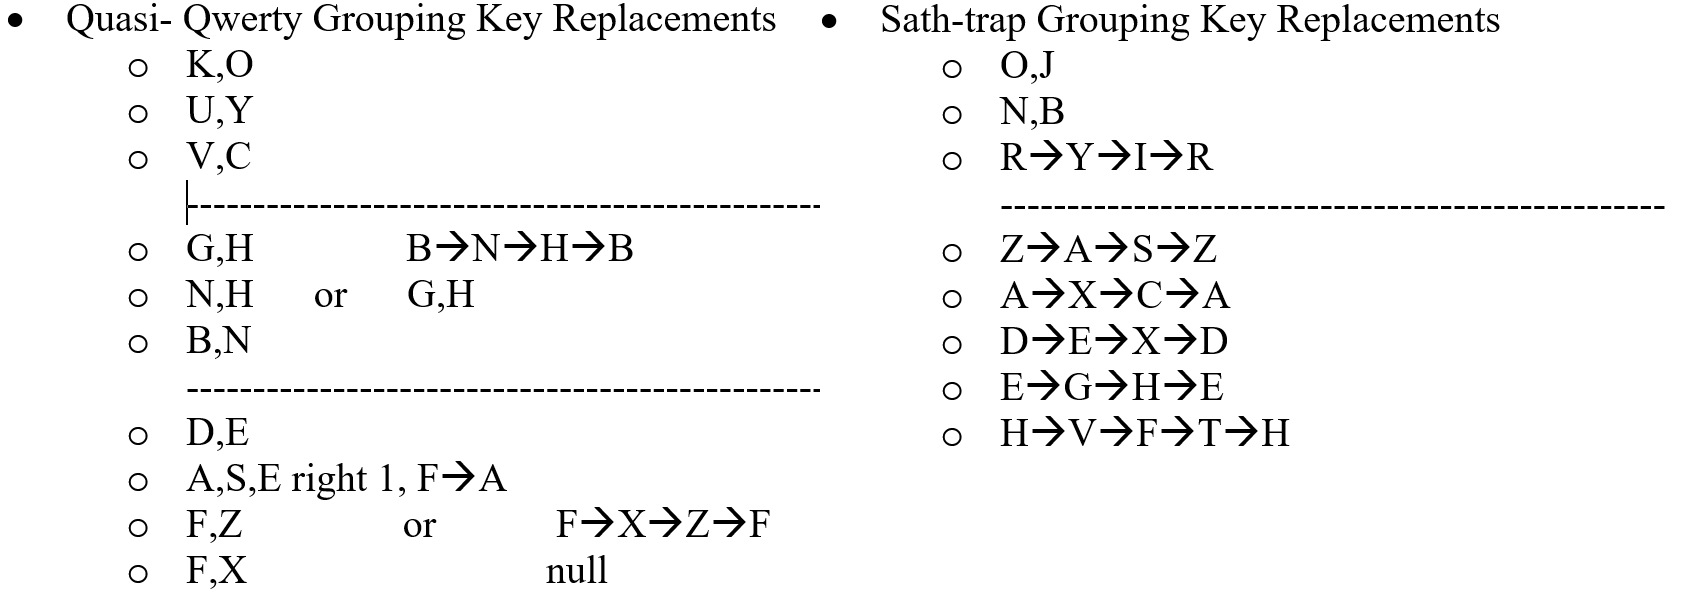
\includegraphics [width=0.8\linewidth]{figures/group1}
	
\end{figure*}

An alternative method we are considering for key replacement is initially moving the vowels to heir place on the new keyboard. Next, we will swap keys to their respective places beginning from Q, in the top left corner, and working our way to M, in the bottom left corner.  Below are the replacements for this method.  


\begin{figure*}[ht]
	\centering
	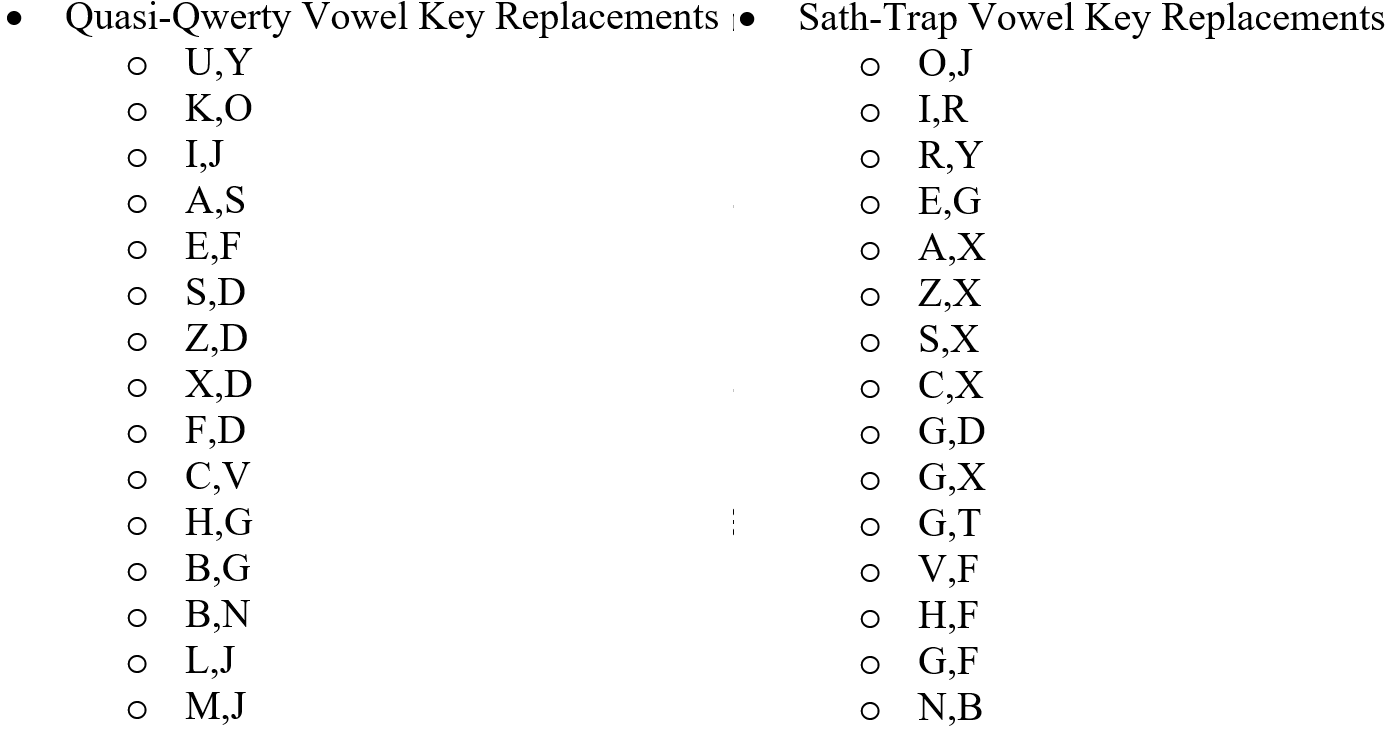
\includegraphics [width=0.7\linewidth]{figures/group2}
	
\end{figure*}


\subsection{Measurement}

The main instrumentation we are using in this study is the keyboard application that we are downloading onto our subjects' phones. In this experiment we are still trying to narrow down what metrics we want to use.  Some of the options discussed are: 

\begin{itemize}
\item Speed in words per minute (WPM)[2].  This measurement regards every five characters typed as one word, including spaces. This measurement includes the length of the transcribed string excluding the first letter, divided by the time in seconds it took to type that string.  Then, multiply by 60 to convert the seconds to minutes and divide by five to convert number of characters to number of ‘words'.  

\item Accuracy (Corrected, uncorrected, or total error rates) [2].  This measurement includes correct characters (C), incorrect and not fixed characters (INF), incorrect and fixed characters (IF) and finally all backspaces used to fix errors (F). Using these variables, you can calculate three different error rates; corrected, uncorrected, and total.  Corrected error rate is IF/(C+INF+IF), uncorrected error rate is INF/(C+INF+IF), and total error rate is the sum of the two.  

\item Error rates can also be measured by Cumulative and Chunk error rates [2].  This method would disallow error correction all together and treated any character out of place as an error.  The use of this measurement would require the users to be copying a display text that is presented to them.  

\item Efficiency measures can include utilized bandwidth, and wasted bandwidth [2]. Utilized bandwidth is the measure of how many correct characters there are in comparison to the whole transcribed string: C/(C+INF+IF+F).  Wasted bandwidth is the opposite: (INF+IF+F) /(C+INF+IF+F).  

\item Efficiency can also be measured in cost per correction (CPC).  This measurement accounts for errors that were made but not noticed immediately.  CPC is defined by (IF+F)/(Corrections).  A correction is the number of consecutive chunks of backspaces and letters.  There can be one correction in a string, and there can be multiple corrections in a string.  

\item Initial Entry Time [6]- The time between when a word is presented on the screen to when the last letter in that word is typed.  This measures the user's ability to find the keys quickly.
\end{itemize} 




% BALANCE COLUMNS
\balance{}

% REFERENCES FORMAT
% References must be the same font size as other body text.
\bibliographystyle{SIGCHI-Reference-Format}
\bibliography{references}

\end{document}

%%% Local Variables:
%%% mode: latex
%%% TeX-master: t
%%% End:
